%%%%%%%%%%%%%%%%%% DO NOT TOUCH THIS FILE %%%%%%%%%%%%%%%%%%%%%% DO NOT TOUCH THIS FILE%%%%%%%%%%%%%%%%%%%%
\documentclass[11pt, twoside]{article} 
% Formatting options
\usepackage[a4paper]{geometry}
\geometry{left=25mm, right=25mm, bottom = 30mm}

\usepackage[utf8]{inputenc}

% positioning of images
\usepackage[export]{adjustbox}
\usepackage{wrapfig}
\usepackage{transparent}
% Apa reference style
% use textcite for in-text references and parencite for parental references
% formatting of hyperlinks for URL coded in blue
\usepackage{url}
\usepackage{hyperref}
% break lines in captions
\usepackage{caption}
%insert pdf to appendix
\usepackage{pdfpages}
% title page
\usepackage{fancyhdr}
\usepackage[dvipsnames]{xcolor}
% define color from university template
\definecolor{uos_red}{RGB}{172, 6, 25}
\definecolor{uos_yellow}{RGB}{251, 185, 0}
\definecolor{uos_greay}{RGB}{207, 207, 207}
\definecolor{cssj_purple}{RGB}{79, 8, 123}
\definecolor{cssj_orange}{RGB}{212, 112, 59}

\hypersetup{colorlinks,
    linkcolor={cssj_purple},
    citecolor={cssj_purple},
    urlcolor={cssj_purple!80!black}
}
% colour package for in-text colour use
\usepackage{eso-pic, graphicx}
% references
\usepackage[natbib=true,backend=biber,sorting=nyt,style=apa,dateabbrev=false]{biblatex}
\renewcommand*{\bibfont}{\fontsize{10}{12}\selectfont}
% add your references to this file
\addbibresource{references.bib}

% colored box packages
\usepackage{tikz,lipsum,lmodern}
\usepackage[most]{tcolorbox}



%------------------HEADER---------------------%
\pagestyle{fancyplain}
\fancyhead[L]{{Implementing Artificial Neural Networks with TensorFlow}}
\fancyhead[R]{{ESBN Transformer}}
\fancyfoot[C]{\thepage}
\renewcommand*\familydefault{\sfdefault} 
%------------------HEADER---------------------%



\begin{document}
\begin{abstract}
While Deep Learning has become increasingly capable over the past years, current models are still lacking key features of human cognition, especially  when it comes to energy and data efficiency. One important component of human reasoning might be the ability to quickly abstract high-level features and perform computations on them. The relational bottleneck \textcite{webb_relational_2023} introduces a form of abstract reasoning into deep learning architectures and has shown high data efficiency on relational reasoning tasks resembling human IQ tests. In this paper, we re-implement the Emergent Symbol Binding Network (ESBN) \textcite{webb_emergent_2021} and evaluate its performance when reducing the key size, a hyperparameter that sets the dimensionality of the abstract representations in the model. In the second part of the paper, incorporate the ESBN into a classical transformer architecture and evaluate its performance on a zero-shot language generalization task. While we were able to reproduce the findings of \textcite{webb_emergent_2021} in the re-implementation part of the study, we did not find significant improvements on the language task when introducing a purely relational processing stream into the transformer both with and without the ESBN.
\end{abstract}

\section{Introduction}
Modern large language models have made great leaps showing near human performance across various benchmarks. However, they typically require vast amounts of training data and computational resources. A recent line of work introduced the so called "relational bottleneck" \textcite{webb_relational_2023} which is a novel way of implementing symbolic processing into deep neural networks without manually defining the symbolic representations. Architectures implementing this bottleneck show superior data efficiency on relational tasks such as ravens progressive matrices, same different relations and distribution of three tasks \textcite{webb_relational_2023}. It has also been shown that these models work extremely well on tasks that require relational as well as semantic processing \textcite{altabaa_abstractors_2023}. \newline
\textcite{russin_compositional_2019} could show that introducing separate information processing streams for relational and semantic information improves model performance on a language based generalization task. 
In this paper, we re-implement the ESBN model by \textcite{webb_emergent_2021} and evaluate the impact of reducing key size on training accuracy. In a second experiment, we integrate the ESBN into a standard transformer \textcite{vaswani_attention_2023} and compare its performance against a transformer and an Abstractor \textcite{altabaa_abstractors_2023} architecture on the language-based generalization task scan \textcite{lake_generalization_2018}.


\section{Distribution-of-Three Experiment}
In the first experiment, we evaluate models on the distribution of three task. The objective of the task is for the model to choose the right image from four possibilities to complement the pattern in the presented data. As in the original study \textcite{webb_emergent_2021}, we use simple Unicode images and generate the data by constructing random subsets. First, we recreate the m = 0 and the m = 95 condition from the original study and after that, we evaluate how decreasing the key size of the model impacts performance on the m = 95 condition.

\subsection{Task}
In this experiment, we consider the distribution-of-three task. The data consists of Unicode images in sequences of nine. The first three images of the sequence represent the pattern. The two following images are contained in the first three images so that there is one image left to complete the pattern. Of the last four images, one is the image necessary to complete the pattern and three are random. The training objective is to select the index of the right image in the last four and can be expressed as a multiple choice task with four possibilities. The order of the images within the pattern does not matter in this task. \newline
We recreate two conditions from the original study. In the m = 0 condition, all of the 100 Unicode images are used both in the train and evaluation data whereas in the m = 95 condition, 95\% of the images are withheld from the training data. This condition is where generalization ability is most challenging for architectures such as the transformer \textcite{vaswani_attention_2023} and the LSTM \textcite{hochreiter_long_1997} as shown in \textcite{webb_emergent_2021}.

\begin{figure}
    \centering
    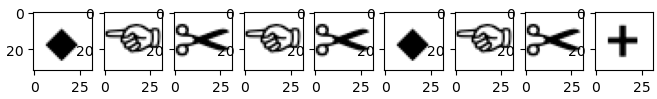
\includegraphics[width=0.8\linewidth]{images/sample_data.png}
    \caption{Sample from Distribution-of-Three layer. In this sample, the diamond, the hand and the scissor form one set. The subsequent two images are hand and scissor such that the image of the diamond remains to complete the set. Thus, the model should output index 0 since this is the index of the correct shape from the last four images.}
    \label{fig:sample_data}
\end{figure}

\subsection{Model}
In this experiment, we do a re-implementation of the ESBN model by \textcite{webb_emergent_2021}. The model has a convolutional encoder that creates 128 dimensional image embeddings. On the embedded image sequence, the model applies temporal context normalization \textcite{webb_learning_2023} as did the authors in the original paper. The embeddings are then passed to the ESBN component of the model that is responsible for the relational processing. The ESBN has an LSTM controller component with a hidden size of 512 and from its output, 256 dimensional keys as well as the four dimensional predictions are produced at each timestep of the sequence. The model output are the last predictions that are derived from the LSTM output using a dense layer with the softmax activation function.

\subsubsection{Emergent Symbol Binding Mechanism}
At the core of the ESBN lie two separate memory stores \(M_k\) and \(M_v\) that grow dynamically when processing one sequence. The keys memorized in \(M_k\) are purely symbolic in nature since they are generated by a LSTM controller that operates only on relational information. The first key in \(M_k\) is generated by feeding in a vector of zeros to the LSTM controller. To compute the subsequent key in \(M_k\), a weighted sum based on similarity scores of the elements in \(M_v\) is passed to the controller. The similarity scores for the weighted sum are calculated via the dot product between the input embeddings stored in \(M_v\) and are passed through a softmax nonlinearity. Additionally, a gain parameter \(g\) is calculated from a dense layer receiving the controller output and concatenated to the LSTM input. This mechanism allows only same-different information to be passed to the controller which is at the core of the relational reasoning capabilities of the network.

\begin{figure}
    \centering
    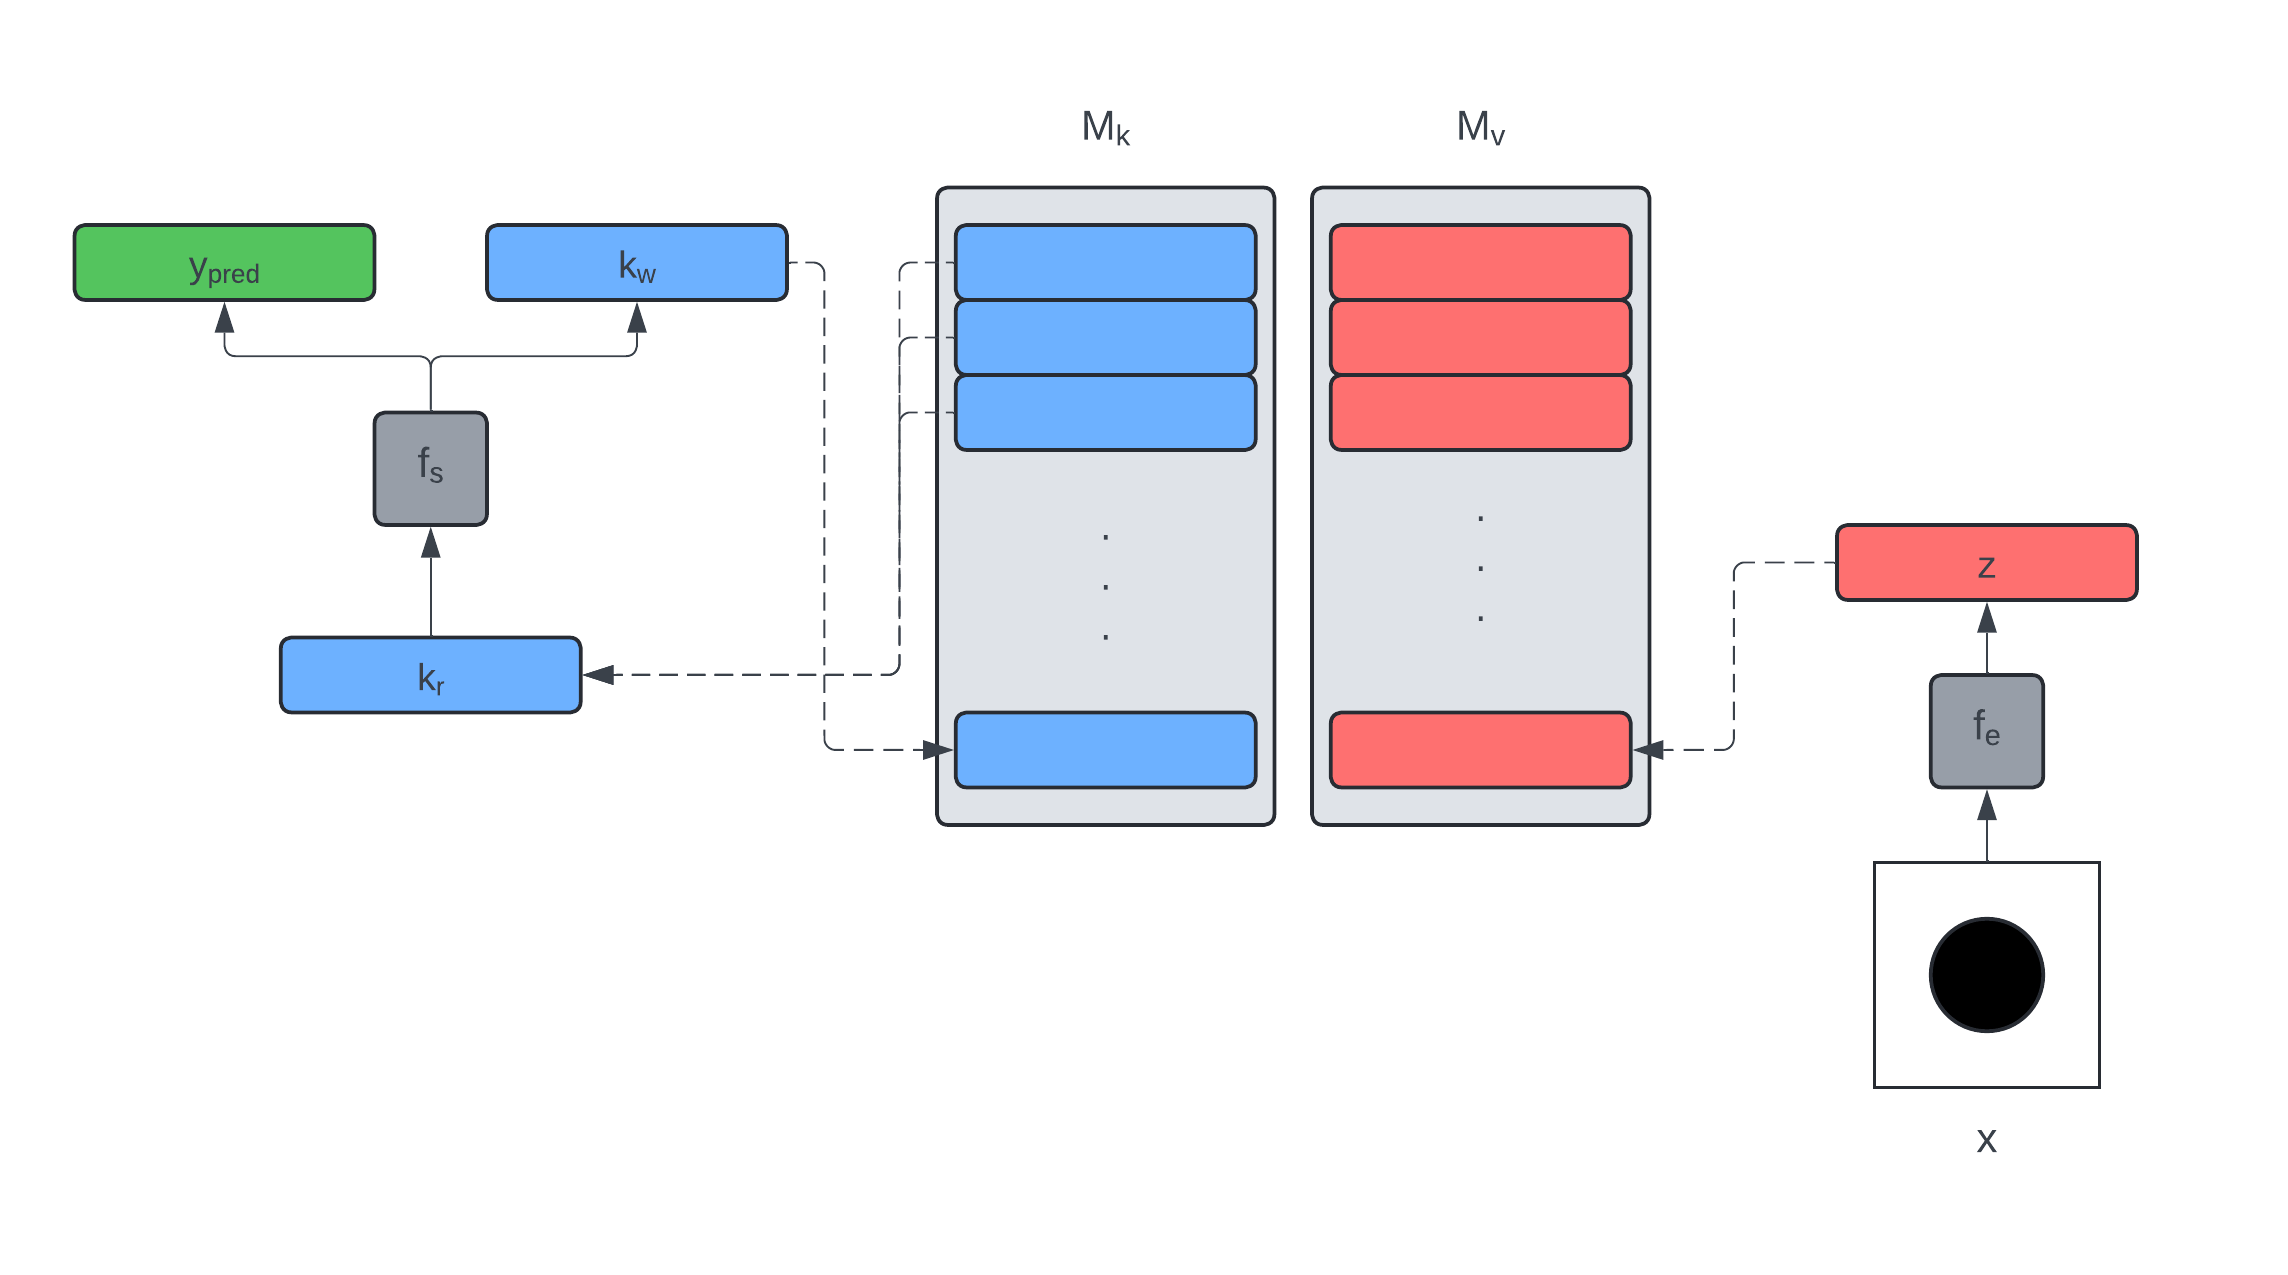
\includegraphics[width=1.0\linewidth]{images/ESBN_Model.png}
    \caption{Emergent Symbol Binding Network as described by \textcite{webb_emergent_2021}. For simplicity, we do not show the dense network computing the gain parameter \(g\) from the LSTM output.}
    \label{fig:esbn_model}
\end{figure}


\subsection{Results}
\subsubsection{Replication Study}
For our replication study, obtain similar results as \textcite{webb_emergent_2021} both for the m = 0 and the m = 95 condition. When evaluating the batch-level accuracy during training, we observe near perfect accuracy after only a some tens of iterations which is exactly what the original paper found as well.

\begin{figure}
    \centering
    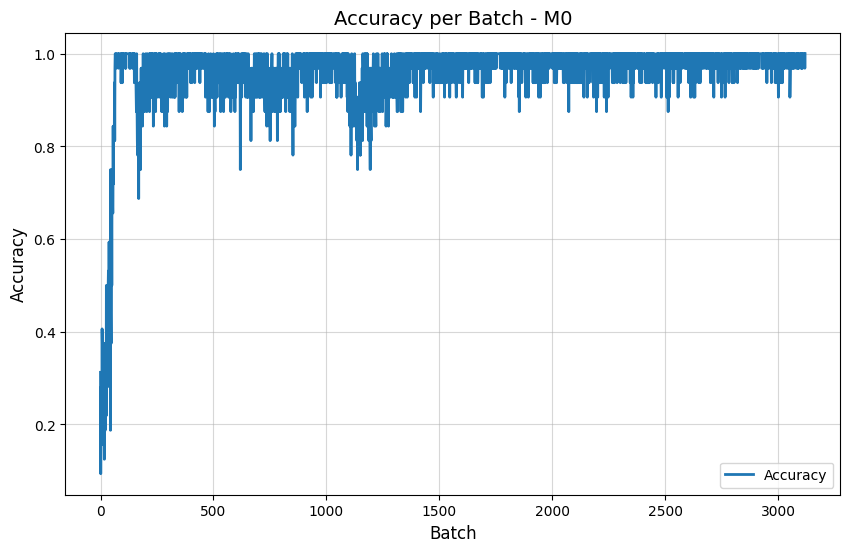
\includegraphics[width=0.6\linewidth]{images/acc_batchlvl_m0.png}
    \caption{Train accuracy of the ESBN model in the m = 0 condition evaluated at the batch level. The plot shows the extremely rapid convergence of the model that was observed in the original study by \textcite{webb_emergent_2021}.}
    \label{fig:acc_batchlvl_m0}
\end{figure}

\begin{figure}
    \centering
    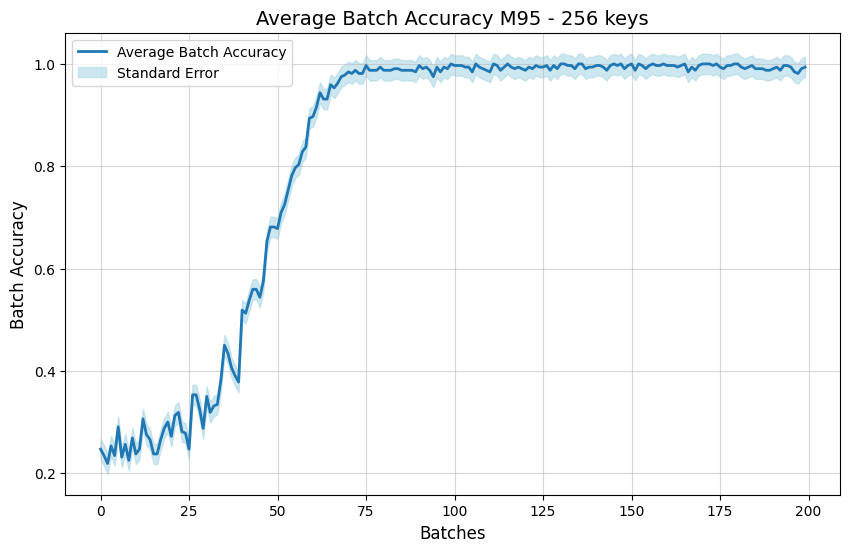
\includegraphics[width=0.6\linewidth]{images/avg_batch_acc_m95_keys256.png}
    \caption{Mean train accuracy of ten train runs on the m = 95 condition with the original key size of 256 evaluated at the batch level.}
    \label{fig:acc_batchlvl_m95}
\end{figure}

\subsection{Key Size Evaluation}
To better understand what impact the key size has on the model performance, we systematically reduced this hyperparameter and compared validation accuracy for different key sizes. The key size is the size of the abstract symbols that the model uses and to better understand the properties of symbolic processing in the ESBN, it is interesting to see how varying this parameters impacts the model. For each condition, we trained ten models and compared the mean performance on the m = 95 condition. \newline

\begin{figure}
    \centering
    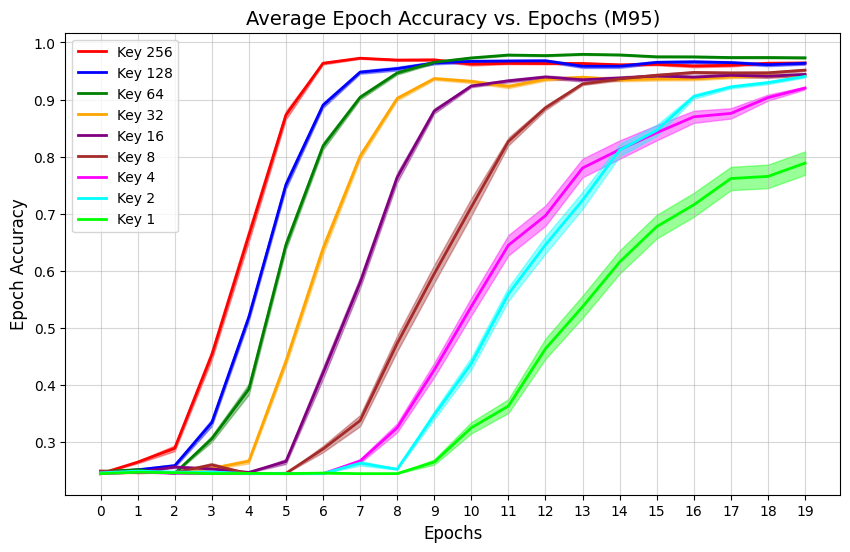
\includegraphics[width=0.8\linewidth]{images/epoch_acc_m95.png}
    \caption{Model performance for different key sizes. Each line corresponds to the mean accuracy of ten models, shaded areas represent the standard error. The results suggest that decreasing the key size decreases the speed of convergence for the model, though the ESBN can tolerate even very small key sizes.}
    \label{fig:epoch_acc_m95}
\end{figure}

\subsection{Discussion}
In the experiment, we successfully replicated the findings from \textcite{webb_emergent_2021}. The network architecture and the rationale behind it might open up interesting areas of research since it is an elegant combination of symbolic processing and bottom-up connectivist procedures. \newline
Decreasing the key size up to a single dimension showed that the symbolic component of the architecture can tolerate extremely small representation sizes, at least for simple tasks. This further demonstrates the capability of the relational bottleneck as it does not necessarily rely on large symbolic representations to perform well. \newline
Also, the symbol binding mechanism is a biologically plausible simplified model of the processes that might happen in human reasoning. The human hippocampus receives highly processed information and it is able to recall associated information from memory. This whole process is modulated by the prefrontal cortex. This mechanism is mirrored by the ESBN whereby the memory components of the model are analogous to the hippocampus and the LSTM corresponds to the prefrontal cortex.
The model is however a huge simplification and human processing is infinitely more complicated. One limitation, for instance, is that the model can only compare embedding via the dot product. In human reasoning, these comparisons should be able to take into account different features of the embeddings depending on the circumstances.\newline
Another weakness of the ESBN model is that the LSTM is not ideal for handling very long sequences as it suffers from vanishing gradients and there are more adequate models that incorporate the relational bottleneck. One such model would be the Abstracter \textcite{altabaa_abstractors_2023} that builds on the transformer and allows symbolic processing to occur on a multitude of positions. \newline
Also, as pointed out by \textcite{webb_relational_2023}, the ESBN can only learn symmetric relations. This can be accounted for by stacking ESBN layers but the Abstracter \textcite{altabaa_abstractors_2023} is capable of learning asymmetric relations directly \textcite{webb_relational_2023}.


\section{Zero-Shot Generalization on Language Tasks}
In this experiment, we use the ESBN to add a purely symbolic processing stream to a transformer. Since the ESBN shows superior performance on relational tasks (Webb 2023) it is plausible to assume that incorporating this architecture into a transformer would aid with generalization capabilities of the model. \newline
One finding in this direction comes from (Russin 2019) who showed that the addition of a purely syntactic processing stream into a recurrent neural network improved the performance of the model on the generalization of language. 

\subsection{Task}
The second experiment concerns the addprim\_jump subset of the scan dataset \textcite{lake_generalization_2018}. The dataset tests models for zero-shot generalization on language tasks. It consists of verbal instructions for walking in different directions and the associated actions. In the addprim\_jump subset, the word "jump" is not used in the instructions in the train set but it is used in the evaluation set. The model thus has to generalize to correctly interpret the word. \newline
Our experiment is motivated by (Russing et. al, 2019) who used the dataset to evaluate generalization of a model that has seperate processing streams for semantics and syntax. Also, \textcite{altabaa_abstractors_2023} introduced the abstractor, a variant of the transformer that can incorporate the relational bottleneck at various positions in a transformer. In the paper, they argue that the standard transformer does in fact use relation based processing but that it entangles symbolic representations with embedding level features.
It would be interesting to see if the ESBN could be used. Currently, large language models have made great leaps in their ability to reason at near human level (CITATIONS). This performance however requires vast amounts of both training data and computational resources. At the same time, the human brain runs on much less energy and is still able to generalize far better than any current AI system with low amounts of data. One possible contribution to this ability is the ability to do relational processing that facilitates abstract reasoning. \newline
One interesting feature

\subsection{Models}

\begin{figure}
    \centering
    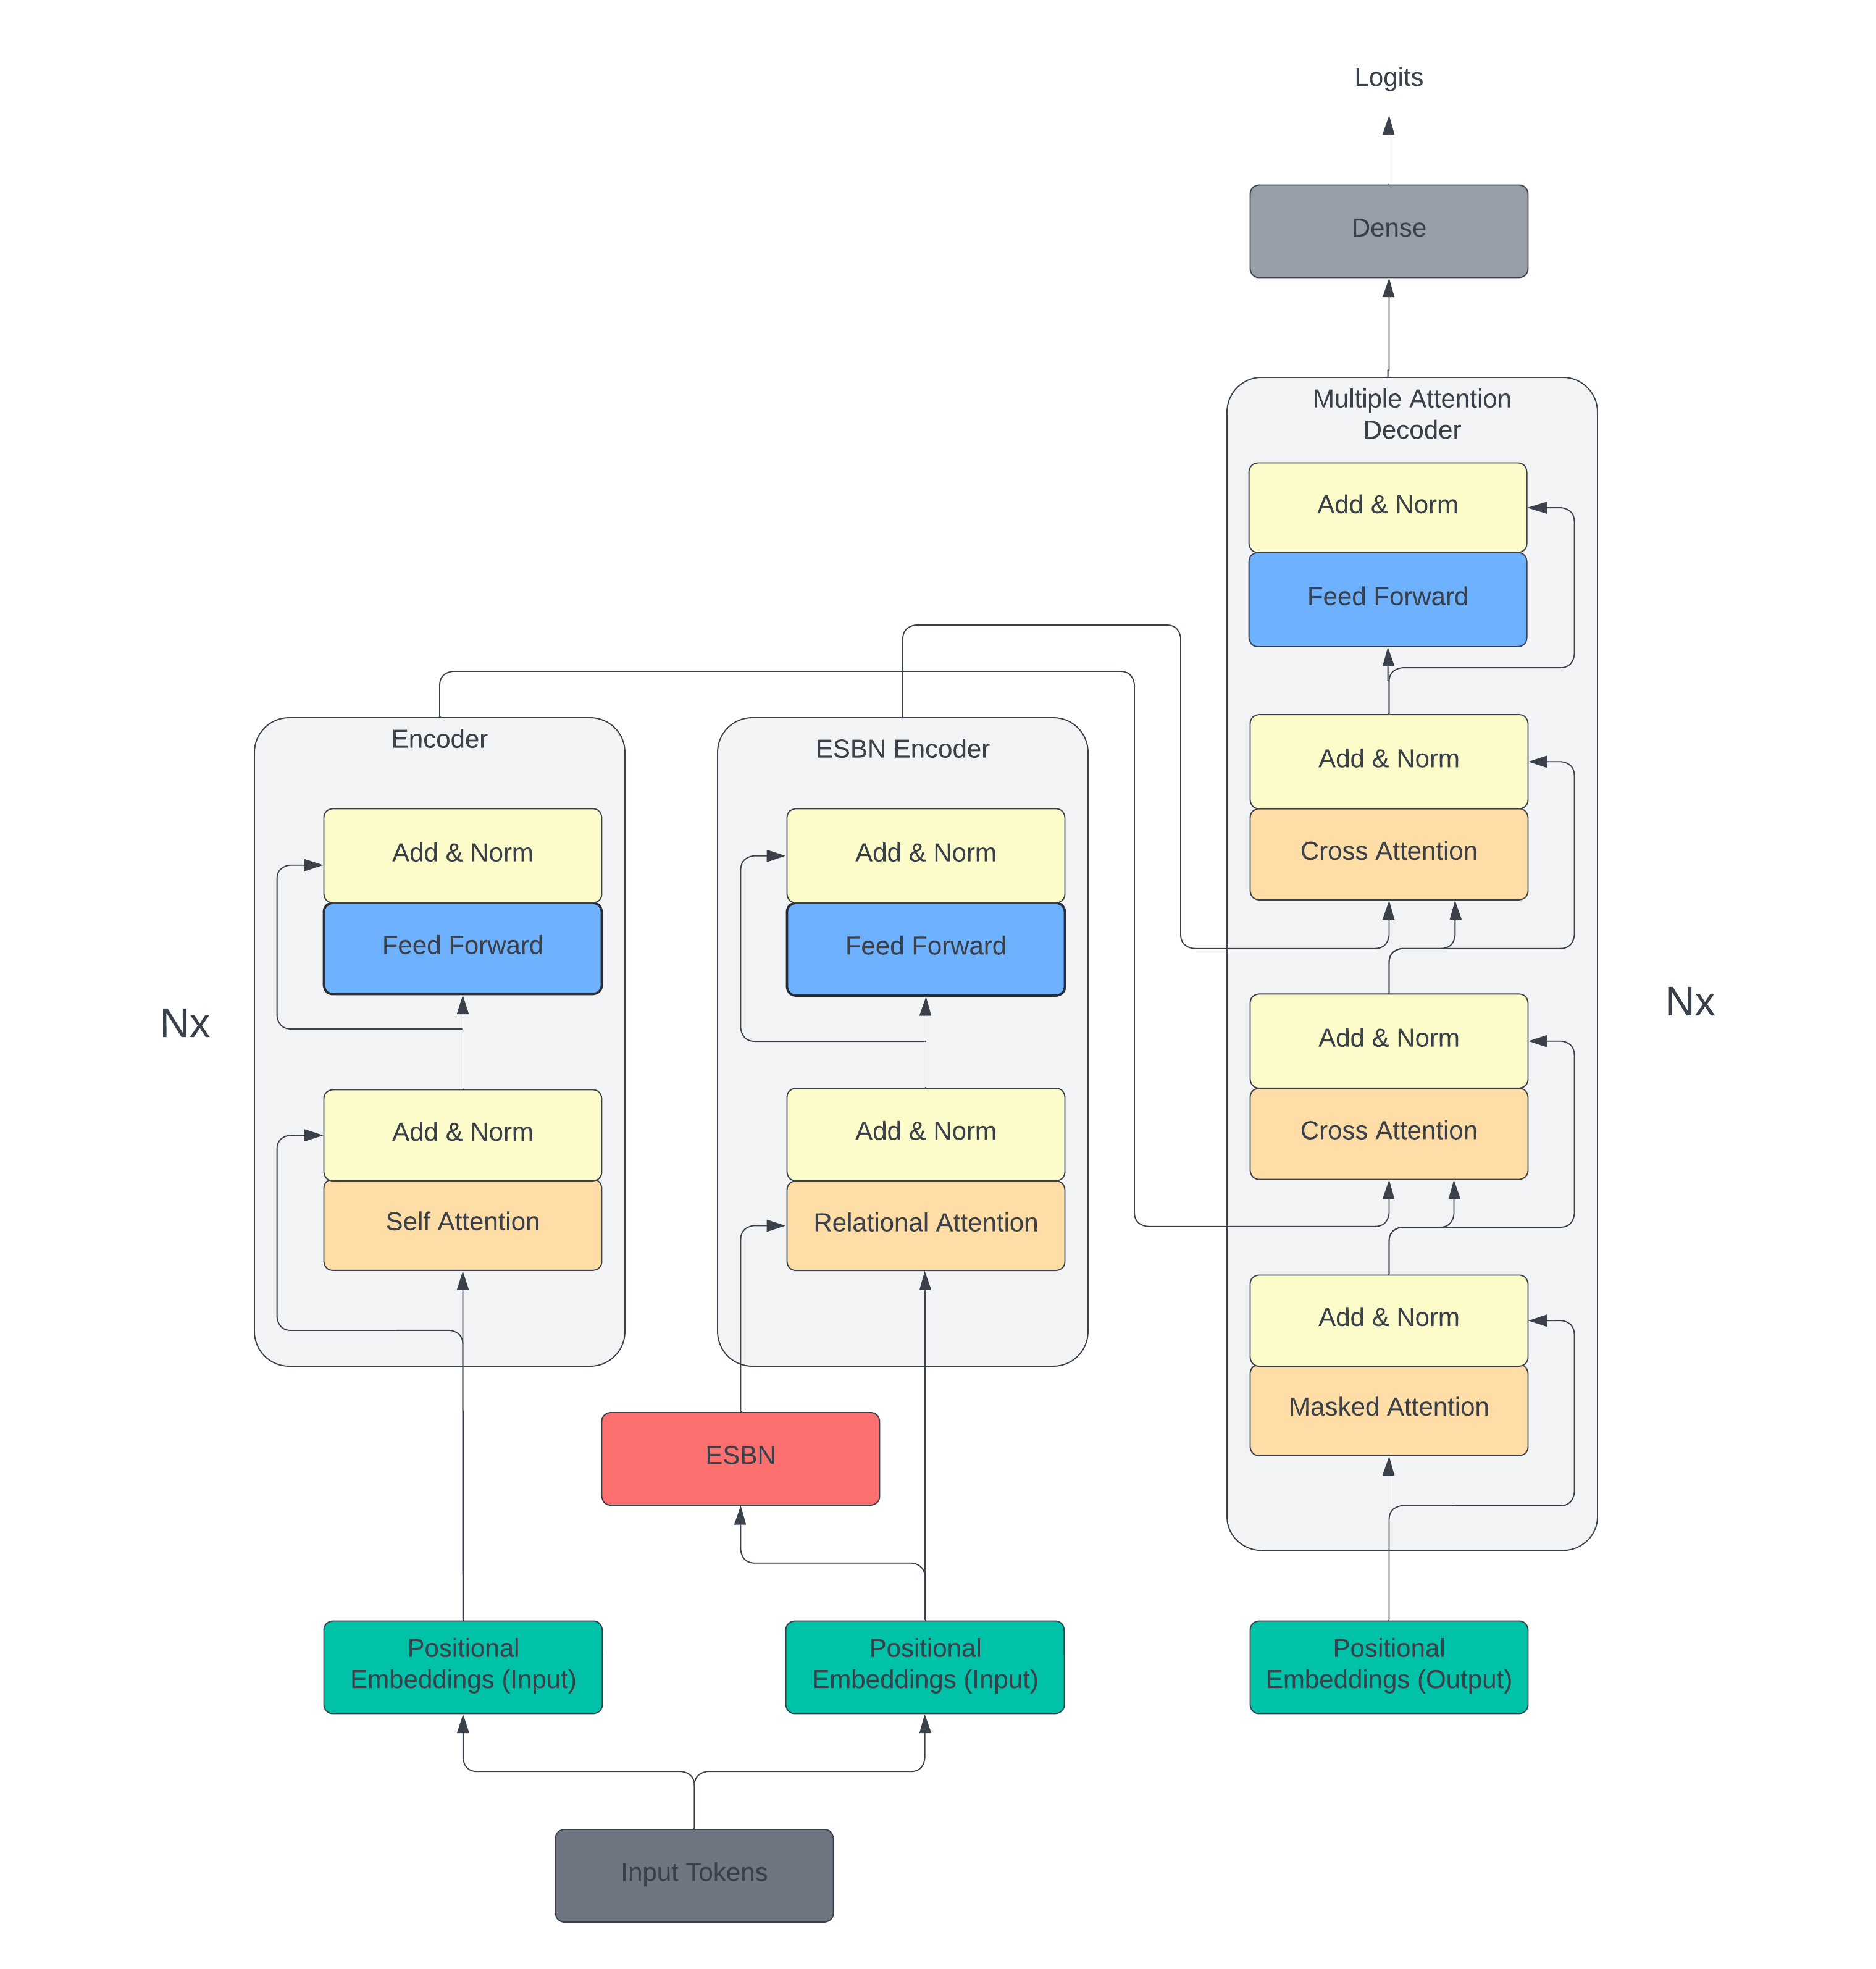
\includegraphics[width=1.0\linewidth]{images/Transformer_Abstracter_ESBN.png}
    \caption{First variant of the transformer. The model has a second encoder that uses relational attention \textcite{altabaa_abstractors_2023} in order to allow for symbolic processing. The symbols are generated by an ESBN layer. The second variant differs only in the symbol generation since it uses learnable parameters as symbols.}
    \label{fig:esbn_transformer}
\end{figure}

The baseline model in this section is a basic transformer \textcite{vaswani_attention_2023} with two layers, a model depth of 32, 4 attention heads and a feed forward dimension of 64. The encoder component of the model creates the context for the decoder from the input commands. The decoder then uses this context to compute the models predictions for the corresponding actions. \newline
We compare this model against two variants that incorporate symbolic processing. The first variant uses an ESBN layer to generate symbols that are processed in a separate Abstracter \textcite{altabaa_abstractors_2023} module. We use a key size of 32 to facilitate later usage of the keys via attention and because Experiment 1 suggested that this dimensionality should not impact the ability to generalize.  \newline 
Thus, the model generates two contexts for the encoder to attend to and for each context, we add a component to the decoder to perform cross-attention. Apart from that, the decoder works like the one introduced in \textcite{vaswani_attention_2023}. The second variant works similar with the difference that symbols are not generated by an ESBN but are a set of learnable parameters of the model as was suggested by \textcite{altabaa_abstractors_2023}.

\subsection{Results}
Due to computational restrictions, we ran only one training script per model with 20 epochs. In our experiment, we did not find significant differences in the average accuracy on the validation data.

\begin{figure}
    \centering
    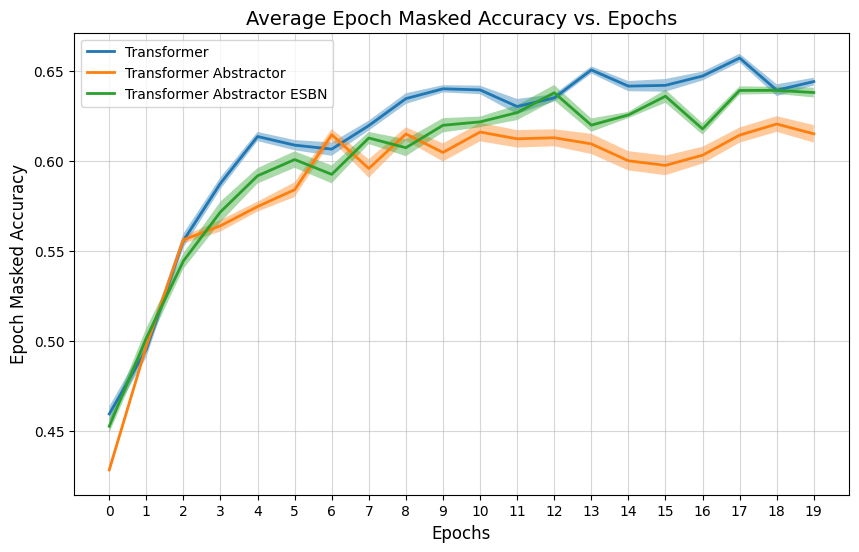
\includegraphics[width=1.0\linewidth]{images/avg_epoch_acc_tf.png}
    \caption{Average Masked Accuracy of the examined models on the scan task. Each model was trained five times, shaded areas show the standard error. }
\end{figure}

\subsection{Discussion}
In our experiment, we did not find any convincing benefits of implementing the ESBN layer into a transformer architecture for generalization. \newline
This might indicate that the transformer already combines relational and non-relational information in a way that suit the task well. As \textcite{altabaa_abstractors_2023} point out, the transformer does indeed intertwine relational and non-relational features due to the attention mechanism used as the dot product between the key and query is a form of the relational bottleneck but the multiplication with the value component re-introduces low-level features. However, at least in our experiment, this might be actually help performance on the task. \newline
Another explanation might be that the transformer does not need to rely on the symbolic component for training since it is already capable provide a near perfect fit for the training data without the symbolic component. So the model might ignore the symbolic information stream during training and does not learn to generalize.


\section{General Discussion}
The ESBN is one of several model architectures that implement the relational bottleneck \textcite{webb_relational_2023}. The idea to include an inductive bias that predisposes the model to extract higher-level abstract features opens up many possibilities to extend generalization of models. One might reason that this ability is central to human cognition and integrating it into artificial neural networks might help both with modeling the human mind as well as improving the models themselves. One hint for the existence of a relational bottleneck in the human brain is the behavior that the ESBN displays in the Give-N-Task. It could be shown that the learning progression of the model, in contrast to other popular architectures, closely resembles the learning progression of actual human children \textcite{webb_emergent_2021} as in \textcite{webb_relational_2023}. \newline 
It remains to be seen how much current language models can benefit from symbolic processing but in our opinion, it could prove to be a powerful tool towards increasing data and computational efficiency of Large Language Models. Though, the ESBN is probably not ideally suited in that regard as it suffers from the same limitations as the LSTM and the memory component increases the required memory. \newline
The Abstracter \textcite{altabaa_abstractors_2023} might be a more elegant choice to improve language models as it incorporates relational processing into transformer architectures more naturally and it is more flexible and memory efficient. 
\printbibliography[]{}
\newpage
\section{Appendix}
\subsection{Code Availability}
All the code used to create the experiments can be accessed via \hyperlink{https://github.com/Jonathank2510/esbn_abstractor/tree/main}{Github}

\subsection{Distribution-of-Three Experiment}
\subsubsection{Dataset Generation}
The dataset generation procedure was adapted from \textcite{webb_emergent_2021} and we generated the datasets from scratch for both the m = 0 and m = 95 condition. For the m = 0 condition, the train set size was 10000, for the m = 95 condition it was 320 since no more permutations can be produced from five shapes. Test set size was 10000 for both condition.
\subsubsection{Hyperparameters}
For the first part of the experiment, we have chosen the same hyperparameters as \textcite{webb_emergent_2021} in order to properly recreate the experiment. The image encoder consists of three convolutional layers with 32 filters each and two dense layers with 256 and 128 units. Both of the dense layers use the relu activation function and we use a simple flatten layer to pass the output of the last convolutional layer to the dense layers. \newline
The original model uses an embedding size of 128, a key size of 256 and a hidden size of 512 for the LSTM controller. \newline
For all conditions, we used the Adam \textcite{kingma_adam_2017} optimizer with a learning rate of 0.001. In the m = 0 condition, we trained for 10 epochs and for the m = 95 condition, we trained for 20 epochs. For all condition, a batch size of 32 was used both for training and evaluation.
\subsubsection{Model evaluation}
For the m = 95 condition, we performed a single training run and evaluated its performance on the batch level. For the key size evaluation, we performed ten training runs for each condition and used the mean and standard deviation of epoch accuracy to compare models.

\subsection{Zero-Shot Generalization on Language Tasks}
\subsubsection{Dataset}
We tested our models on the addprim\_jump split of the scan \textcite{lake_generalization_2018} dataset. The dataset consists of 14,670 examples for training and 7,706 for evaluation.
\subsubsection{Hyperparameters}
All the models had two layers, an embedding depth of 32, 64 units in the feed forward layers and four attention heads. For each attention block, we used dropout with a rate of 0.1. Also, we use layer normalization and addition of residual connections for better trainability. \newline
We trained for 20 epochs using the Adam \textcite{kingma_adam_2017} optimizer with a learning rate of 0.001 and a batch size of 32.
\subsection{Model evaluation}
We evaluated the mean masked accuracy for five training runs for each model.

\end{document}
